\def\year{2018}\relax
%File: formatting-instruction.tex
\documentclass[letterpaper]{article} %DO NOT CHANGE THIS
\usepackage{aaai18}  %Required
\usepackage{times}  %Required
\usepackage{helvet}  %Required
\usepackage{courier}  %Required
\usepackage{url}  %Required
\usepackage{graphicx}  %Required
\graphicspath{ {images/} }
\frenchspacing  %Required
\setlength{\pdfpagewidth}{8.5in}  %Required
\setlength{\pdfpageheight}{11in}  %Required
%PDF Info Is Required:
  \pdfinfo{
/Title (Sentence Summarization Using a Worker-Supervisor Approach)
/Author (Zhou Zhou)}
\setcounter{secnumdepth}{0}  
 \begin{document}
% The file aaai.sty is the style file for AAAI Press 
% proceedings, working notes, and technical reports.
%
\title{Sentence Summarization Using a Worker-Supervisor Approach}
\author{Zhou Zhou\\
Rose-Hulman Institute of Technology\\
5500 Wabash Avenue\\
Terre Haute, IN 47803\\
}
\maketitle
\begin{abstract}
In this paper, I created a sentence-level summarization system using neural networks and an abstractive approach. The work is based on the NAMAS system Facebook created, with extensions and a novel training method to improve its performance. The direction of improvement points to teaching the model about words or phrases that share similar meanings, making it possible to infer proper summarizations despite of lack of training data otherwise.
\end{abstract}

\section{Introduction}
Sequence-to-sequence neural systems have been considered a hard problem because word dependencies can be long with huge chunks of texts, and models are either stable against noise or efficiently trainable, but not both \cite{bengio1994learning}. In recent years, the field of language modeling has seen dramatic improvements in many aspects, especially in terms of machine translation models. Recurrent Neural Networks, Long Short-Term Memory, attention module, and the encoder-decoder structure, all are part of the reasons machine translation models performing phenomenally better than before.

However, it’s not just the machine translation tasks get performed better. Language modeling is essential to many Natural Language Processing tasks, one of which is sentence summarization. As there are more tools in the toolbox, significant innovations and improvements are observed in this field as well.

In this paper, we present the work to combine techniques from state-of-the-art sentence summarization models and neural machine translation systems. We propose the worker-supervisor architecture, where the worker can be any existing or new sequence-to-sequence system and the supervisor can be any RNN that outputs a single values as a score. It is inspired by the "Read-Again" strategy in which the encoder is fed the source sentence twice before proceeding to decoding. It is also comparable to Generative Adversarial Network (GAN), which has the notion of generator and discriminator. The discriminator tells whether a given input is human-generated or not, and the generator tries to trick the discriminator into thinking its output is human-generated (whereas it is generated by a neural network). The latter architecture has also shown promising results in generation tasks such as image and music generation.

\section{Related Work}
The work of this research stems directly from that of Facebook researchers have done. Their first system achieved abstractive sentence summarization using an attention-based encoder, a beam search based decoder, and a generation algorithm \cite{rush2015neural}. Later on, researchers at Facebook worked further on improving the model. First, they improved the way of training the model. Instead of training the model with ground truth data, they used generated data to train the rest of the network \cite{ranzato2015sequence}. On the other hand, a group of joint researchers from Tsinghua University and University of Toronto employed a “Read-Again” strategy, scanning the input two times to point the attention better. They also developed a copy mechanism to copy words from input to output, so rare words can be simply copied over, resulting in a smaller vocabulary size \cite{zeng2016efficient}. Although their groups have different research directions, both groups pointed out that their work has been based on the work of neural machine translation methods, mostly from Bengio et al \cite{bahdanau2014neural}. This shows the connection between the sentence summarization task and the machine translation task. In fact, one can think of sentence summarization as a special form of machine translation, where the source language and the target language are the same. This makes it important to also consider the recent developments in the field of machine translation using neural network as well.

After the invention of Long Short-Term Memory, the vanishing gradient problem for RNNs was mediated \cite{sutskever2014sequence}. This allowed further innovations to follow up. \cite{bahdanau2014neural} created a successful system using bidirectional RNN as the encoder of the input sentence. However, a great breakthrough was made by Google Brain researchers \cite{johnson2016google}. They used a deep LSTM network with 8 layers as the encoder and another 8 layers as the decoder. Moreover, they used residual connections in the encoder and an attention mechanism in the decoder. This created the phenomenon of “Zero-Shot Translation”, where the model can learn to translate between language pair A and C given only data on language pair A and B and language pair B and C. Another way to obtain a system that can do zero-shot translation is to use a pivot language as the intermediate language B at training time, where the model is trained on language pair A and B, and B and C, which has also been shown to be effective \cite{chen2017teacher}. Some researchers also attempted to tackle the drawbacks of an artificial evaluation method. Yang, Zhen, et al. built a generative adversarial network where the discriminator grades the output instead of using an artificial evaluation function (such as BLEU) \cite{yang2017improving}. Given that sequence-to-sequence models tend to be very large, attempts were also made to reduce the training time of a large network, such as the Mixture-of-Experts layer that avoids training unused portion of the network given a specific input \cite{shazeer2017outrageously}. Lastly, to overcome the issues of the model forgetting the rare words that have only a few occurrences, Feng, Yang, et al. augmented their model with a memory that maps source words that have rare occurring frequencies to their translations \cite{feng2017memory}.

\section{Model Architecture}
We combine the idea of the encoder-decoder architecture with a custom Read-Again strategy, and propose the worker-supervisor architecture. In this architecture, the worker produces the summarized text using the given input. This initial output is concatenated with the original input, and the combined text is then fed into the supervisor to determine whether the summary is acceptable. If the supervisor decides against this summary, the summary is then fed back into the worker so the worker can read both the original input and its own original output, and come up with a new summary, hopefully of better quality than the original. This process may repeat for a given number of times. We will describe the architecture of this architecture in details below.

This idea is derived from the "Read-Again" strategy, where the source sentence is read twice before outputting the summary. The researchers believed it worked better because showing the source sentence twice allow dependencies to form from beginning parts of the sentence to the later parts of the sentence. Without seeing the sentence twice, only dependencies from later parts of the sentence to the beginning parts of the sentence can be formed. The same rationale is used to justify the proposal of bi-directional RNNs []. Therefore, we decided to allow dependencies to form between the source sentence and the last attempted summary. This is to mimic how human correct a summary. When one is told his or her summary is not good enough, he or she will compare the summary with the source sentence to determine what was not good enough, and produce a revised summary based on that. Since the attention mechanism has provided the ability to focus on parts of the input, in which case can help comparing only parts of the source sentence and the summary, we think this is a way to mimic the human process of correcting a summary.

\subsection{Worker}
A worker should be itself a full sequence-to-sequence model that can generate summary with or without a supervisor. As any existing text summarization model should be able to take this role, we picked Google’s GNMT model as the worker [5]. GNMT uses 8 LSTM layers with 1024 units on either side, with the encoder using residual connections and the encoder using the attention mechanism. These features have allowed GNMT to perform well in translation tasks, even between multiple language pairs. This capacity should be more than enough to take on the summarization task, which is between one language pair in which both the source language and the target language are the same.

\subsection{Supervisor}
A supervisor should also be an RNN to be able to read a sequence with arbitrary length. It can be simpler than the worker though, as it does not need to generate text outputs. Instead, it should generate a score to describe how much it thinks a concatenated text contains an acceptable summary. We used 8 normally-stacked LSTM layers with 1024 units and a fully connected layer connected to the last layer. The fully connected layer has only one output, and uses the sigmoid function as its activation function to guarantee an output between 0 and 1.

\subsection{Embedding}
Embedding layers are used to convert each text token (in the form of an integer value) into a vector of some representation []. This process takes place before the input is fed into the encoder, the decoder, and the supervisor. A well trained embedding would generate the representation based on the meaning of the word, so sometimes it would place synonyms in spatially close locations. In a machine translation task, separate embeddings are used by the encoder and the decoder, so one may naturally question, since we are using the same source and target language, do we need two embeddings or one? We decided to go with two embeddings, because the task of the decoder is significantly different from the encoder, and it might need different information from its inputs.

\begin{figure}[h]
	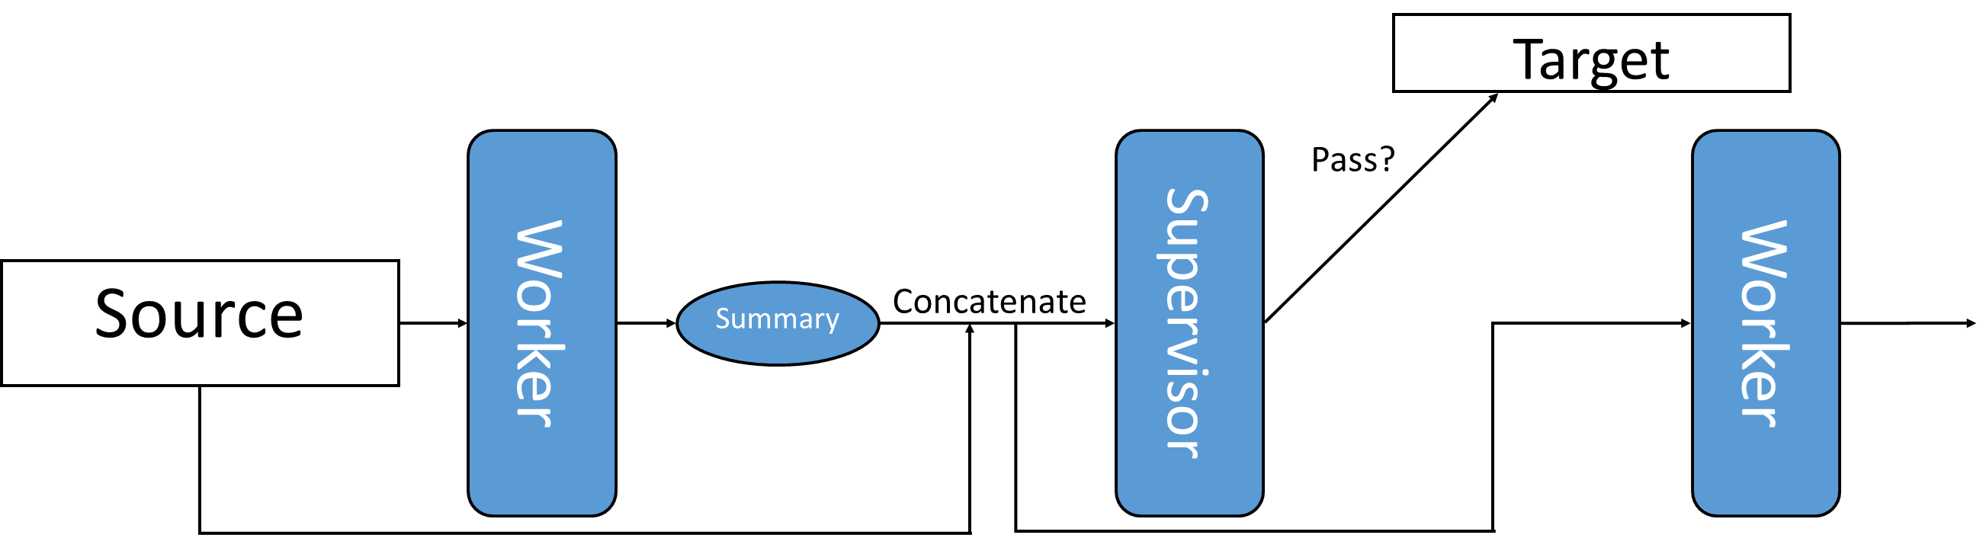
\includegraphics[scale=0.2]{architecture}
	\centering
	\caption{The worker-supervisor architecture}
\end{figure}

\subsection{Training the Model}
We train the model with the following procedure:
\begin{itemize}
	\item The worker is trained with a batch of sentence pairs from the training set.
	\item The supervisor is trained with a batch consisting of concatenated input and output sentence and a score of 0.99. We are not using 1 because using extreme values (0 and 1) during training time is not preferred in GAN training [].
	\item The worker is run to get a batch of inferred sentences.
	\item These sentences are concatenated with their source sentences, then sent to the supervisor with a score of 0.01.
	\item These sentences are paired up with the actual target sentences, and then sent to the worker to train it.
\end{itemize}
For instance, if one sentence pair in the dataset is the following:
\begin{center}
	source: a yale school of medicine study is expanding upon what scientists know about the link between schizophrenia and nicotine addiction .\\
	target: researchers examining evidence of link between schizophrenia and nicotine addiction
\end{center}

We first train the worker on this sentence pair. Then we run the worker to generate a summary of the source sentence:
\begin{center}
	summary: yale study links schizophrenia
\end{center}
We then concatenate this sentence with the source sentence, with a start of sentence token in-between to mark the start of the summary. Then we have created this training sentence pair (<sos> denotes the start of sentence token):\\
\begin{center}
	source: a yale school of medicine study is expanding upon what scientists know about the link between schizophrenia and nicotine addiction . <sos> yale study links schizophrenia\\
	target: researchers examining evidence of link between schizophrenia and nicotine addiction
\end{center}

Then we train the worker again with this sentence pair. After both sentence pairs have been trained on the worker, we move on to the next sentence pair in the dataset.

\subsection{Running the Model}
The way to run the model is different than training because we allow the worker to retry the work multiple times, and a threshold score is used to determine whether the summarization needs to be redone.
\begin{itemize}
	\item The worker runs on the input sentence to generate an initial summary.
	\item The summary and the input sentence are concatenated and sent to the supervisor to obtain a score.
	\item If a score is greater than a specified threshold, then output the summary.
	\item Otherwise, the concatenated sentence is sent back to worker and repeat the steps above. These steps will only execute for at most a specified number of times.
\end{itemize}

\section{Environment Setup}
We used the Annotated English Gigaword corpus [] as the training dataset, and DUC 2003 and 2004 as the evaluation set. We followed the same preprocessing step as in the published NAMAS project []. We selected this preprocessing method because it has built-in tokenization and filters out bad article titles that do not constitute a summary of the first sentence of that article.

We selected the GNMT system built as the worker, and a multi-layer RNN with a fully-connected layer at the end as the supervisor. The worker is built with TensorFlow and the supervisor is built using Keras with a TensorFlow backend. The encoder and decoder of GNMT and the supervisor have 8 layers of LSTM cells. We selected the batch size as 8 and spread the model across 8 GPUs. When concatenating sentences, we chose to retain the SOS token and the EOS token, because we thought these were clues for the encoder to realize this is a rework of a summarized sentence. During inference, we selected the rework threshold to be 0.5 and the maximum retries to be 10.

\section{Results}

\section{Discussions}

\section{Conclusion}

\bibliography{References}
\bibliographystyle{aaai}
\end{document}
